\documentclass{article}

% if you need to pass options to natbib, use, e.g.:
%     \PassOptionsToPackage{numbers, compress}{natbib}
% before loading neurips_2019

% ready for submission
 \usepackage{neurips_2019, times}
% to compile a preprint version, e.g., for submission to arXiv, add add the
% [preprint] option:
     %\usepackage[preprint]{neurips_2019}

% to compile a camera-ready version, add the [final] option, e.g.:
%   \usepackage[final]{neurips_2019}

% to avoid loading the natbib package, add option nonatbib:
%     \usepackage[nonatbib]{neurips_2019}

\usepackage[utf8]{inputenc} % allow utf-8 input
\usepackage[T1]{fontenc}    % use 8-bit T1 fonts
\usepackage{hyperref}       % hyperlinks
\usepackage{url}            % simple URL typesetting
\usepackage{booktabs}       % professional-quality tables
\usepackage{amsfonts}       % blackboard math symbols
\usepackage{nicefrac}       % compact symbols for 1/2, etc.
\usepackage{microtype}      % microtypography
\usepackage{graphicx}

\usepackage{floatrow}
\newfloatcommand{capbtabbox}{table}[][\FBwidth]
\usepackage{blindtext}

\usepackage{geometry}
\usepackage{amsmath}
\usepackage{cancel}

\newcommand{\bM}{\mathbf{M}}
\newcommand{\bv}{\mathbf{v}}
%\newcommand{\be}{\mathbf{e}}
\newcommand{\bI}{\mathbf{I}}

\title{Numerical Stable SVD}

% The \author macro works with any number of authors. There are two commands
% used to separate the names and addresses of multiple authors: \And and \AND.
%
% Using \And between authors leaves it to LaTeX to determine where to break the
% lines. Using \AND forces a line break at that point. So, if LaTeX puts 3 of 4
% authors names on the first line, and the last on the second line, try using
% \AND instead of \And before the third author name.

\author{%
  David S.~Hippocampus\thanks{Use footnote for providing further information
    about author (webpage, alternative address)---\emph{not} for acknowledging
    funding agencies.} \\
  Department of Computer Science\\
  Cranberry-Lemon University\\
  Pittsburgh, PA 15213 \\
  \texttt{hippo@cs.cranberry-lemon.edu} \\
  % examples of more authors
  % \And
  % Coauthor \\
  % Affiliation \\
  % Address \\
  % \texttt{email} \\
  % \AND
  % Coauthor \\
  % Affiliation \\
  % Address \\
  % \texttt{email} \\
  % \And
  % Coauthor \\
  % Affiliation \\
  % Address \\
  % \texttt{email} \\
  % \And
  % Coauthor \\
  % Affiliation \\
  % Address \\
  % \texttt{email} \\
}

\begin{document}

\maketitle

\begin{abstract}
Singular Value Decomposition (SVD) has been widely used in deep learning, and matrix backpropagation algorithm is applied to compute the gradients. However, matrix backpropagation is numerically unstable as it involves the computation of reciprocal of the difference of arbitrary pair of eigenvalues which will cause overflow if the difference between the two eigenvalues are very small. In this paper, we propose to employ Power Iteration (PI) method to approximate the gradients of SVD during backpropagation. It can be proved that when the iteration number of PI goes to infinite, the gradients computed via PI will equal to the gradients of SVD. In other words, the gradients computed via PI can be viewed as the geometric series expansion of the gradients of SVD. The experimental results demonstrate that the proposed method, which uses SVD as forward pass and PI as backward pass, is more stable than SVD or PI. Besides, we also employs the numerically stable SVD to design a denoising layer by removing small eigenvalues during reconstruction, and it can boost the performance of the network.
\end{abstract}

\section{Problem}
SVD has accurate and stable forward pass. However, it has accurate but \textbf{numerical unstable} gradients.

\section{PCA Denoising Layer}
Options to implement PCA Norm Layer.
\begin{itemize}
\item Given input covariance matrix $\bM$, use \textbf{Eigen Decomposition} or \textbf{Singular Value Decomposition (SVD)} Operation as forward computation, and use the analytic solution of its gradient for backward propogation.
\item Given input covariance matrix $\bM$, vectors with random values $[\bv_1^{1}, \bv_2^{1}, ...]$, use \textbf{Power Iteration} as forward computation, and use its gradient for backward propogation.
\item Given input covariance matrix $\bM$, vectors with random values $[\bv_1^{1}, \bv_2^{1}, ...]$, use \textbf{Eigen Decomposition} or \textbf{SVD} Operation as forward computation, and use \textbf{Power Iteration} to approximate the analytic solutions of the gradient for backward propogation.
\end{itemize}

Usually, people choose either option 1 or option 2 to implement PCA Norm Layer, but both of them have problems.
In option 1, \textbf{Eigen Decomposition} or \textbf{Singular Value Decomposition (SVD)}, the analytic solutions of the gradient sometimes causes NaN problem when there are two or more eigenvalues are too close to each other.
In option 2, if the two eigenvalues are very close, eigenvectors could not be computed precisely with limited power iteration number. Thus, during backprorogation, the derivatives will be very inaccurate and destroy the parameters of model, and cause numerical instability in the training process.

In this paper, we propose to using option 3. During forward pass, we use \textbf{SVD} to compute the eigenvalues. 
SVD is numerically more stable than eigendecomposition \cite{nakatsukasa2013stable} as SVD implementation employs a divide-and-conquer strategy, while the eigendecomposition uses QR algorithm. 
During backpropogation, we employ \textbf{Power Iteration} method to compute the numerical solutions of the covariance matrix $\bM$ gradient.
In \textbf{sections} \ref{sec: pi} \& \ref{sec: mbp}, we will prove that when the iteration number goes to infinite, the accumulated gradients (\emph{i.e.} numerical solution) from the \textbf{Power Iteration} method is exactly the same with the analytic solution of the gradient.


\newpage

\section{Approximate SVD gradient with Power Iteration in backpropogation}
In the following 2 subsections, we will prove that when the gradient computed from Power Iteration equals to the gradients computed from SVD.
	\subsection{Gradient of Power Iteration}
	\label{sec: pi}
	To compute the leading eigenvector $\bv$ of $\bM$, Power Iteration uses the following standard formula,
	\begin{equation}
	\bv^{(k)} = \frac{\bM\bv^{(k-1)}}{\| \bM\bv^{(k-1)} \|},
	\end{equation}
	in which $\| {\cdot} \|$ denotes the $l_2$ norm, and $v^{(0)}$ is usually initialized randomly with  $\|v^{(0)}\|{=}1$.
    Its gradient formula is as follows~\cite{ye2017dynamic},
	\begin{equation}
	\begin{aligned} 
	\frac{\partial L}{\partial \bM} &=\sum_{k} \frac{\left(\bI-\bv^{(k+1)} \bv^{(k+1)\top}\right)}{\left\|\bM \bv^{(k)}\right\|} \frac{\partial L}{\partial \bv^{(k+1)}} \bv^{(k)\top} \\
	\frac{\partial L}{\partial \bv^{(k)}} &=\bM \frac{\left(\bI-\bv^{(k+1)} \bv^{(k+1)\top}\right)}{\left\|\bM \bv^{(k)}\right\|} \frac{\partial L}{\partial \bv^{(k+1)}} 
	\end{aligned}
	\end{equation}
	Using 3 power iteration steps for demonstration.
	\begin{equation}
	\begin{aligned} 
	\frac{\partial L}{\partial \bv^{(2)}} &=\bM \frac{\left(\bI-\bv^{(3)} \bv^{(3)\top}\right)}{\left\|\bM \bv^{(2)}\right\|} \frac{\partial L}{\partial \bv^{(3)}}\\
	\frac{\partial L}{\partial \bv^{(1)}} &=\bM \frac{\left(\bI-\bv^{(2)} \bv^{(2)\top}\right)}{\left\|\bM \bv^{(1)}\right\|} \frac{\partial L}{\partial \bv^{(2)}}
	=\bM \frac{\left(\bI-\bv^{(2)} \bv^{(2)\top}\right)}{\left\|\bM \bv^{(1)}\right\|} 
	\bM \frac{\left(\bI-\bv^{(3)} \bv^{(3)\top}\right)}{\left\|\bM \bv^{(2)}\right\|} \frac{\partial L}{\partial \bv^{(3)}}
	\end{aligned}
	\end{equation}
	
	Then the $\frac{\partial L}{\partial \bM}$ should be like the following, for the reason that we use eigenvalue decomposition (ED)'s result, denoted as $\bv$ as initial value, then $\bv {=} \bv^{(0)} {\approx}\bv^{(1)} {\approx} \bv^{(2)}{\approx} \cdots {\approx}\bv^{(k)}$. 
	
	\begin{equation}
	\begin{aligned} 
	\frac{\partial L}{\partial \bM}
	&{=}\frac{\left(\bI-\bv^{(3)} \bv^{(3)\top}\right)}{\left\|\bM \bv^{(2)}\right\|} \frac{\partial L}{\partial \bv^{(3)}} \bv^{(2)\top} +
	\frac{\left(\bI-\bv^{(2)} \bv^{(2)\top}\right)}{\left\|\bM \bv^{(1)}\right\|} \frac{\partial L}{\partial \bv^{(2)}} \bv^{(1)\top} + 
	\frac{\left(\bI-\bv^{(1)} \bv^{(1)\top}\right)}{\left\|\bM \bv^{(0)}\right\|} \frac{\partial L}{\partial \bv^{(1)}} \bv^{(0)\top}\\
	&{=} \left( \frac{\left(\bI {-} \bv \bv^{\top}\right)}{\left\|\bM \bv\right\|} {+}
	 \frac{\left(\bI {-} \bv \bv^{\top}\right) \bM  \left(\bI {-} \bv \bv^{\top}\right)}{\left\|\bM \bv\right\|^{2}}  {+} 
	 \frac{\left(\bI {-} \bv \bv^{\top}\right) \bM \left(\bI {-} \bv \bv^{\top}\right) \bM \left(\bI {-} \bv \bv^{\top}\right)}{\left\|\bM \bv\right\|^{3}} \right)
	 \frac{\partial L}{\partial \bv^{(3)}} \bv^{\top}
	\end{aligned}
	\label{eq: pi_expand}
	\end{equation}
	
	Known that $\bv \bv^{\top}$ and $\bM$ are symmetric and $\bM \bv = \lambda \bv$, we have 
$$\bv\bv^{\top}\bM = (\bM^{\top}\bv\bv^{\top})^{\top} = (\bM\bv\bv^{\top})^{\top} = (\lambda\bv\bv^{\top})^{\top} = \lambda\bv\bv^{\top} = \bM\bv\bv^{\top}.$$
	Introducing the equation above into the numerator in the second term of Eq.\ref{eq: pi_expand}, we can obtain:
	\begin{equation}
	\begin{aligned}
	\left(\bI - \bv \bv^{\top}\right) \bM  \left(\bI - \bv \bv^{\top}\right) &
	= \left(\bM - \bv \bv^{\top}\bM\right) \left(\bI - \bv \bv^{\top}\right) 
	=  \left(\bM - \bM \bv \bv^{\top}\right) \left(\bI - \bv \bv^{\top}\right) \\
	= \bM \left(\bI - \bv \bv^{\top}\right) \left(\bI - \bv \bv^{\top}\right) &
	= \bM \left(\bI - 2\bv \bv^{\top} + \bv \cancel{\left(\bv^{\top}\bv \right)} \bv^{\top}\right) 
	= \bM \left(\bI - \bv \bv^{\top} \right).
	\end{aligned}
	\label{eq: term1}
	\end{equation}
	Similarly, for the numerator in the third term in Eq.\ref{eq: pi_expand}, we have:
	\begin{equation}
	\left(\bI - \bv \bv^{\top}\right) \bM \left(\bI - \bv \bv^{\top}\right) \bM \left(\bI - \bv \bv^{\top}\right) = \bM \bM \left(\bI - \bv \bv^{\top} \right).
	\label{eq: term2}
	\end{equation}
	
Introducing Eq.\ref{eq: term1} and Eq.\ref{eq: term2} into Eq.\ref{eq: pi_expand}, we can obtain	
	\begin{equation}
	\frac{\partial L}{\partial \bM}
	 = \left( \frac{\left(\bI-\bv \bv^{\top}\right)}{\left\|\bM \bv\right\|} +
	 \frac{\bM \left(\bI-\bv \bv^{\top}\right)}{\left\|\bM \bv\right\|^{2}}  + 
	 \frac{\bM \bM \left(\bI-\bv \bv^{\top}\right)}{\left\|\bM \bv\right\|^{3}} \right)
	 \frac{\partial L}{\partial \bv^{(3)}} \bv^{\top}
	\label{eq: pi_3iter}
	\end{equation}

Extending the iteration number from 3 to $k$, Eq.\ref{eq: pi_expand} will be extended as
	\begin{equation}
	\frac{\partial L}{\partial \bM}
	 = \left( \frac{\left(\bI-\bv \bv^{\top}\right)}{\left\|\bM \bv\right\|}  +
	 \frac{\bM \left(\bI-\bv \bv^{\top}\right)}{\left\|\bM \bv\right\|^{2}}  + \cdots +
	 \frac{\bM^{k-1} \left(\bI-\bv \bv^{\top}\right)}{\left\|\bM \bv\right\|^{k}} \right) \frac{\partial L}{\partial \bv^{(k)}}
	\bv^{\top}
	\label{eq: pi_pytorch}
	\end{equation}	

Eq.\ref{eq: pi_pytorch} is the form we adopt to compute the gradients of SVD, and we set $k{=}19$.

\subsection{Proof of Gradient Equivalence Between Power Iteration and SVD}
In this subsection, we are going to prove that the gradients of SVD and Power Iteration are equivalent. In the end of this section, we can observe that when the number of the iterations goes to infinity, the gradients of Power Iteration can be written as the same form as the one of SVD.

	\begin{equation}
	\begin{aligned}
	\left\|\bM\bv\right\| & = \lambda, \; 
		\left\|\bM\bv\right\|^{2} {=} \lambda^{2}, \cdots, \; 
		\left\|\bM\bv\right\|^{k} {=} \lambda^{k} \\
	\bM &= \lambda_{1}\bv_{1}\bv_{1}^{\top} + \lambda_{2}\bv_{2}\bv_{2}^{\top} + \cdots +  \lambda_{n}\bv_{n}\bv_{n}^{\top}\\
	\bM^{2} &=  (\lambda_{1}\bv_{1}\bv_{1}^{\top} + \lambda_{2}\bv_{2}\bv_{2}^{\top} + \cdots)   (\lambda_{1}\bv_{1}\bv_{1}^{\top} + \lambda_{2}\bv_{2}\bv_{2}^{\top} + \cdots)\\
	 &= \lambda_{1}^{2}\bv_{1}\bv_{1}^{\top}\bv_{1}\bv_{1}^{\top} +  \lambda_{2}^{2}\bv_{2}\bv_{2}^{\top}\bv_{2}\bv_{2}^{\top} + \cdots
	\cancel{\lambda_{1}\lambda_{2}\bv_{1}\bv_{1}^{\top}\bv_{2}\bv_{2}^{\top}} + \cancel{\lambda_{1}\lambda_{2}\bv_{2}\bv_{2}^{\top}\bv_{1}\bv_{1}^{\top}} + \cdots\\
	 &= \lambda_{1}^{2}\bv_{1}\bv_{1}^{\top} +  \lambda_{2}^{2}\bv_{2}\bv_{2}^{\top} + \cdots + \lambda_{n}^{2}\bv_{n}\bv_{n}^{\top}, \\ 
	 \bM^{k} &= \lambda_{1}^{k}\bv_{1}\bv_{1}^{\top} +  \lambda_{2}^{k}\bv_{2}\bv_{2}^{\top} + \cdots + \lambda_{n}^{k}\bv_{n}\bv_{n}^{\top},\\
	\end{aligned}
	\label{eq: term_k}
	\end{equation}
	in which $\bv = \bv_1$ is the leading eigenvector and $\lambda=\lambda_1$ is the leading eigenvalue.
	By introducing Eq.\ref{eq: term_k} into Eq.\ref{eq: final-form}, the derivative can be further formulated as
	
	\begin{equation}
	\begin{aligned} 
	\frac{\partial L}{\partial \bM}
	& =\left( \frac{\left(\bI-\bv_1 \bv_1^{\top}\right)}{\left\|\bM \bv_1\right\|}  +
	 \frac{\bM \left(\bI-\bv_1 \bv_1^{\top}\right)}{\left\|\bM \bv_1\right\|^{2}}  + \cdots +
	 \frac{\bM^{k-1} \left(\bI-\bv_1 \bv_1^{\top}\right)}{\left\|\bM \bv_1\right\|^{k}} \right)
	 \frac{\partial L}{\partial \bv_1^{(k)}}\bv_1^{\top} \\
	&=\left( \frac{\left(\bI-\bv_1 \bv_1^{\top}\right)}{\left\|\bM \bv_1\right\|} +
	\frac{\left(\bM-\lambda \bv_1 \bv_1^{\top}\right)}{\left\|\bM \bv_1\right\|^2}  + \cdots +
	\frac{\left(\bM^{k-1} - \lambda^{k-1}\bv_1\bv_1^{\top}\right)}{\left\|\bM \bv\right\|^{k}} \right) \frac{\partial L}{\partial \bv_1^{(k)}} \bv_1^{\top}\\
	&=\left( \frac{\left(\sum_{i=2}^{n}\bv_{i}\bv_{i}^{\top}\right)}{\lambda_1}      +
	\frac{\left(\sum_{i=2}^{n}\lambda_{i}\bv_{i}\bv_{i}^{\top}\right)}{ \lambda_{1}^{2}} +  \cdots +
	\frac{\left(\sum_{i=2}^{n}\lambda_{i}^{k-1}\bv_{i}\bv_{i}^{\top}\right)}{\lambda_{1}^{k}} \right) \frac{\partial L}{\partial \bv_1^{(k)}}
	\bv^{\top}\\
	&=\left(\sum_{i=2}^{n}\left(
	\frac{1}{\lambda_{1}} +
	\frac{1}{\lambda_{1}}\left(\frac{\lambda_{i}}{\lambda_{1}}\right)^{1} +
	\frac{1}{\lambda_{1}}\left(\frac{\lambda_{i}}{\lambda_{1}}\right)^{2} + \cdots +
	\frac{1}{\lambda_{1}}\left(\frac{\lambda_{i}}{\lambda_{1}}\right)^{k-1}
	\right)\bv_{i}\bv_{i}^{\top}
	\right)\frac{\partial L}{\partial \bv_{1}^{(k)}}\bv_{1}^{\top}\\
	\end{aligned}
	\label{eq: geo-prog-series}
	\end{equation}
	In Eq.\ref{eq: geo-prog-series}, we have a geometric progression series.
	Given that $${1 - (\frac{\lambda_{i}}{\lambda_{1}})^k \rightarrow 1}, \text{when} \; k\rightarrow\infty, \vert \frac{\lambda_{i}}{\lambda_{1}} \vert<1,$$
	then we have
	\begin{equation}
	\frac{1}{\lambda_{1}} +
	\frac{1}{\lambda_{1}}\left(\frac{\lambda_{i}}{\lambda_{1}}\right)^{1} +
	\frac{1}{\lambda_{1}}\left(\frac{\lambda_{i}}{\lambda_{1}}\right)^{2} + \cdots +
	\frac{1}{\lambda_{1}}\left(\frac{\lambda_{i}}{\lambda_{1}}\right)^{k-1} = \frac{\frac{1}{\lambda_{1}}(1- (\frac{\lambda_{i}}{\lambda_{1}})^k)} {1 - \frac{\lambda_{i}}{\lambda_{1}}} 
	\rightarrow  \frac{\frac{1}{\lambda_{1}}}
	{1 - \frac{\lambda_{i}}{\lambda_{1}}}, \text{when} \; k\rightarrow\infty.
	\label{eq: geo-prog-series-deduction}
	\end{equation}
	
	Introducing Eq.\ref{eq: geo-prog-series-deduction} to Eq.\ref{eq: geo-prog-series}, we can obtain	
	\begin{equation}
	\frac{\partial L}{\partial \bM}
	=\left(\sum_{i=2}^{n}\left(
	\frac{\frac{1}{\lambda_{1}}}
	{1 - \frac{\lambda_{i}}{\lambda_{1}}}
	\right)
	\bv_{i}\bv_{i}^{\top}
	\right)\frac{\partial L}{\partial \bv_{1}^{(k)}}\bv_{1}^{\top}
	=\left(\sum_{i=2}^{n}
	\frac{\bv_{i}\bv_{i}^{\top}}
	{\lambda_{1} - \lambda_{i}}
	\right)\frac{\partial L}{\partial \bv_{1}^{(k)}}\bv_{1}^{\top}
	\label{eq: final-form}
	\end{equation}
	
	\subsection{Matrix Back-propagation}
	\label{sec: mbp}
	The analytic soltions of the gradients are from matrix back-propagation~\cite{ionescu2015matrix}.
	\begin{equation}
	\begin{aligned}
	\frac{\partial L}{\partial M}=V\left\{\left(\tilde{K}^{\top} \circ\left(V^{\top} \frac{\partial L}{\partial V}\right)\right)+\left(\frac{\partial L}{\partial \Sigma}\right)_{d i a g}\right\} V^{\top}
	\end{aligned}
	\end{equation}
	
	\begin{equation}
	\begin{aligned}
	\tilde{K}_{i j}=\left\{\begin{array}{ll}{\frac{1}{\lambda_{i}-\lambda_{j}},} & {i \neq j} \\ {0,} & {i=j}\end{array}\right.
	\end{aligned}
	\end{equation}
	
	\begin{equation}
	\begin{aligned}
	\tilde{K} = 
	\begin{bmatrix}
	0  &\frac{1}{\lambda_{1} - \lambda_{2}} &\frac{1}{\lambda_{1} - \lambda_{3}} &\cdots &\frac{1}{\lambda_{1} - \lambda_{n}}\\
	\frac{1}{\lambda_{2} - \lambda_{1}} &0 &\frac{1}{\lambda_{2} - \lambda_{3}} &\cdots &\frac{1}{\lambda_{2} - \lambda_{n}}\\
	\frac{1}{\lambda_{3} - \lambda_{1}} &\frac{1}{\lambda_{3} - \lambda_{2}} &0 &\cdots &\frac{1}{\lambda_{3} - \lambda_{n}}\\
	\vdots &\vdots &\vdots &\ddots &\vdots\\
	\frac{1}{\lambda_{n} - \lambda_{1}} &\frac{1}{\lambda_{n} - \lambda_{2}} &\frac{1}{\lambda_{n} - \lambda_{3}} &\cdots &0
	\end{bmatrix}
	\end{aligned}
	\end{equation}
	where $\lambda_{i}$ is the eigen-value.
	
	\begin{equation}
	\begin{aligned}
	V = 
	\begin{bmatrix}
	\bv_{1} &\bv_{2} &\bv_{3} &\cdots &\bv_{n}
	\end{bmatrix}
	\end{aligned}
	\end{equation}
	where $v_{i}$ is the eigen-vector.
	
	\begin{equation}
	\begin{aligned}
	\frac{\partial L}{\partial V} = 
	\begin{bmatrix}
	\frac{\partial L}{\partial \bv_{1}} &\frac{\partial L}{\partial \bv_{2}}  &\frac{\partial L}{\partial \bv_{3}}  &\cdots &\frac{\partial L}{\partial \bv_{n}} \\
	\end{bmatrix}^{\top}
	\end{aligned}
	\end{equation}
	
	\begin{equation}
	\begin{aligned}
	V^{\top}\frac{\partial L}{\partial V} = 
	\begin{bmatrix}
	\bv_{1}^{\top}\frac{\partial L}{\partial \bv_{1}} &\bv_{1}^{\top}\frac{\partial L}{\partial \bv_{2}}  &\bv_{1}^{\top}\frac{\partial L}{\partial \bv_{3}}  &\cdots &\bv_{1}^{\top}\frac{\partial L}{\partial \bv_{n}} \\
	\bv_{2}^{\top}\frac{\partial L}{\partial \bv_{1}} &\bv_{2}^{\top}\frac{\partial L}{\partial \bv_{2}}  &\bv_{2}^{\top}\frac{\partial L}{\partial \bv_{3}}  &\cdots &\bv_{2}^{\top}\frac{\partial L}{\partial \bv_{n}} \\
	\bv_{3}^{\top}\frac{\partial L}{\partial \bv_{1}} &\bv_{3}^{\top}\frac{\partial L}{\partial \bv_{2}}  &\bv_{3}^{\top}\frac{\partial L}{\partial \bv_{3}}  &\cdots &\bv_{3}^{\top}\frac{\partial L}{\partial \bv_{n}} \\
	\vdots &\vdots &\vdots &\ddots &\vdots\\
	\bv_{n}^{\top}\frac{\partial L}{\partial \bv_{1}} &\bv_{n}^{\top}\frac{\partial L}{\partial \bv_{2}}  &\bv_{n}^{\top}\frac{\partial L}{\partial \bv_{3}}  &\cdots &\bv_{n}^{\top}\frac{\partial L}{\partial \bv_{n}} \\
	\end{bmatrix}
	\end{aligned}
	\end{equation}
	
	\begin{equation}
	\begin{aligned}
	\tilde{K}\circ V^{\top}\frac{\partial L}{\partial V} = 
	\begin{bmatrix}
	0& \frac{1}{\lambda_{2} - \lambda_{1}}\bv_{1}^{\top}\frac{\partial L}{\partial \bv_{2}}  
	&\frac{1}{\lambda_{3} - \lambda_{1}}\bv_{1}^{\top}\frac{\partial L}{\partial \bv_{3}}  
	&\cdots &\frac{1}{\lambda_{n} - \lambda_{1}}\bv_{1}^{\top}\frac{\partial L}{\partial \bv_{n}} \\
	\frac{1}{\lambda_{1} - \lambda_{2}}\bv_{2}^{\top}\frac{\partial L}{\partial \bv_{1}} &0  
	&\frac{1}{\lambda_{3} - \lambda_{2}}\bv_{2}^{\top}\frac{\partial L}{\partial \bv_{3}}  &\cdots 
	&\frac{1}{\lambda_{n} - \lambda_{2}}\bv_{2}^{\top}\frac{\partial L}{\partial \bv_{n}} \\
	\frac{1}{\lambda_{1} - \lambda_{3}}\bv_{3}^{\top}\frac{\partial L}{\partial \bv_{1}} 
	&\frac{1}{\lambda_{2} - \lambda_{3}}\bv_{3}^{\top}\frac{\partial L}{\partial \bv_{2}}  &0  &\cdots 
	&\frac{1}{\lambda_{n} - \lambda_{3}}\bv_{3}^{\top}\frac{\partial L}{\partial \bv_{n}} \\
	\vdots &\vdots &\vdots &\ddots &\vdots\\
	\frac{1}{\lambda_{1} - \lambda_{n}}\bv_{n}^{\top}\frac{\partial L}{\partial \bv_{1}} 
	&\frac{1}{\lambda_{2} - \lambda_{n}}\bv_{n}^{\top}\frac{\partial L}{\partial \bv_{2}} 
	 &\frac{1}{\lambda_{3} - \lambda_{n}}\bv_{n}^{\top}\frac{\partial L}{\partial \bv_{3}}  &\cdots &0 \\
	\end{bmatrix}
	\end{aligned}
	\end{equation}
	
	We do not use eigenvalues in the forward pass, so that it has no gradients, which means $\frac{\partial L}{\partial \Sigma}=0$.
	Now let's consider the partial derivative \emph{w.r.t} $\bv_{i}$ and ignore $\frac{\partial L}{\partial \bv_{i}}, i \neq 1$.
	Then $\frac{\partial L}{\partial M}$ would be,
	
	\begin{equation}
	\begin{aligned}
	\frac{\partial L}{\partial M}&=
	\begin{bmatrix}
	\sum_{i=2}^{n}\frac{1}{\lambda_{1}-\lambda_{i}}\bv_{i}\bv_{i}^{\top}\frac{\partial L}{\partial \bv_{1}}
	&\cancel{term_2} &\cancel{term_3} &\cdots &\cancel{term_n}
	\end{bmatrix}V^{\top}
	+ \cancel{V\left(\frac{\partial L}{\partial \Sigma}\right)_{d i a g} V^{\top}}\\
	&=\sum_{i=2}^{n}\frac{1}{\lambda_{1}-\lambda_{i}}\bv_{i}\bv_{i}^{\top}\frac{\partial L}{\partial \bv_{1}}\bv_{1}^{\top}
	\end{aligned}
	\end{equation}

Now we have shown that the partial derivative of \emph{e.g.}, $\bv_1$ computed from Power Iteration and SVD share the same form when $k\rightarrow \inf$.
Similar deductions could be done for  $\bv_i, i=2,3,...$.
This justifies that we could use power iteration method during backpropogation to approximate the gradients of SVD, but we need to choose an approximate iteration number.

\subsection{Number of Power Iterations}

\begin{figure}[!htb]
\begin{center}
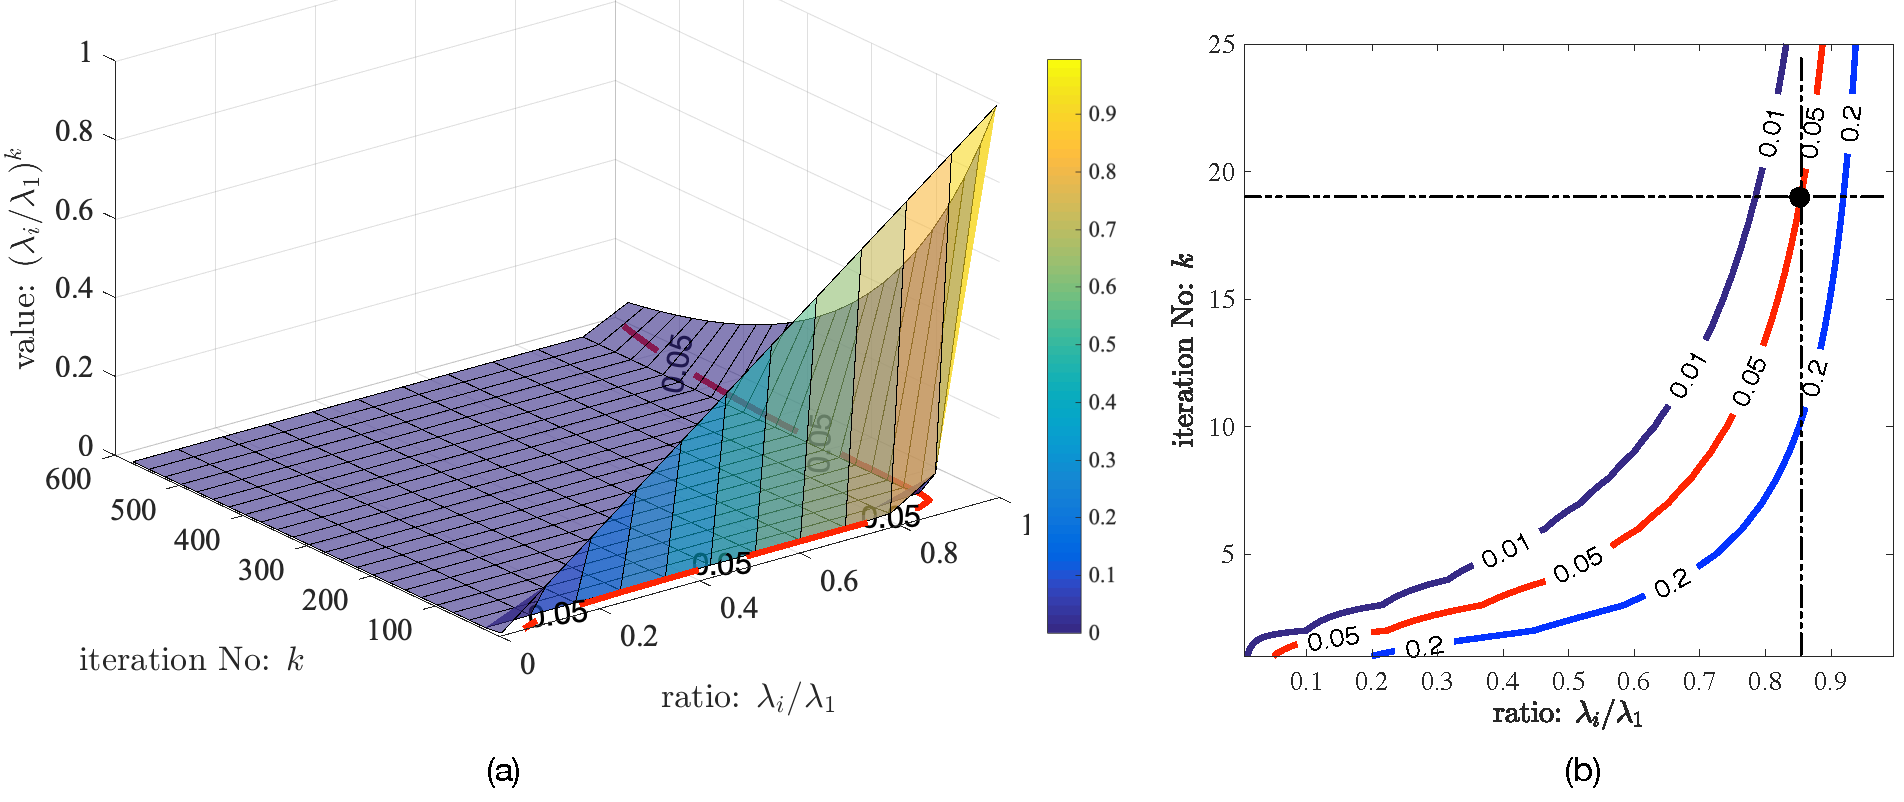
\includegraphics[width=\linewidth]{ratio-k.pdf}
\end{center}
\caption{(a) shows how the value of $(\lambda_k/\lambda_1)^k$ changes \emph{w.r.t.} the eigenvalue ratio $\lambda_k/\lambda_1$ and iteration number $k$. (b) shows the contour of curved surface in (a).}
\label{fig: curve}
\end{figure}

Fig. \ref{fig: curve} shows how the value of $(\lambda_i/\lambda_1)^k$ evolves with different power iteration number $k$ and ratio~$\lambda_i/\lambda_1$. We need to select appropriate $k$ for different $\lambda_i/\lambda_1$ given $(0 < \lambda_i/\lambda_1 \leq 1)$. 

Let's assume $(\lambda_i/\lambda_1)^k<0.05$ being a good approximation to $(\lambda_i/\lambda_1)^k=0$. Then we have
\begin{equation}
(\lambda_i/\lambda_1)^k<0.05 \Leftrightarrow k\; \text{ln}(\lambda_i/\lambda_1) < \text{ln}(0.05) \Leftrightarrow k \geq \frac{\text{ln}(0.05)}{\text{ln}(\lambda_i/\lambda_1)}.
\end{equation}
The minimum value of $k$ to satisfy $(\lambda_i/\lambda_1)^k<0.05$ is $k = \lceil \frac{\text{ln}(0.05)}{\text{ln}(\lambda_i/\lambda_1)} \rceil$.

\begin{table}[!htb]
\begin{center}
\setlength\tabcolsep{4pt}
\begin{tabular}{ccccccccccccccc}
\hline
$\lambda_i/\lambda_1$ & 0.1& 0.2& 0.3 & 0.4 & 0.5 & 0.6 & 0.7 & 0.8 & \textbf{0.85} & 0.9 & 0.95 & 0.99 & 0.995 & 0.999 \\ \hline
$k = \lceil \frac{\text{ln}(0.01)}{\text{ln}(\lambda_i/\lambda_1)} \rceil $   & 2 & 2 & 3 & 4 & 5 & 6 & 9 & 14  & \textbf{19}   & 29  & 59   & 299  & 598   & 2995  \\ \hline
\end{tabular}
\caption{The minimum value of $k$ we need to guarantee $(\lambda_i/\lambda_1)^k<0.05$.}
\label{tab: kmin}
\end{center}
\end{table}

Table \ref{tab: kmin} shows the minimum number of iterations we need to guarantee that the assumption holds. We can observe that when the two eigenvalues are very close to each other \emph{e.g.}, $\lambda_i/\lambda_1=0.999$, we need about 3000 iterations to achieve a good approximation. However, in practice, the case is very rare, and we set power iteration number to be 19. This will satisfy most of the cases. Besides, two very close eigenvalues usually leads to overflow according to Eq.\ref{eq: final-form} as the denominator $\lambda_1 - \lambda_i$ would be close to 0, but with our approximation, this problem could be avoided, and our method is more numerical stable.

\subsection{Percentage of Preserved Information VS Performance}

\begin{figure}[!htb]
\begin{floatrow}
\ffigbox[1.1\FBwidth]{%
  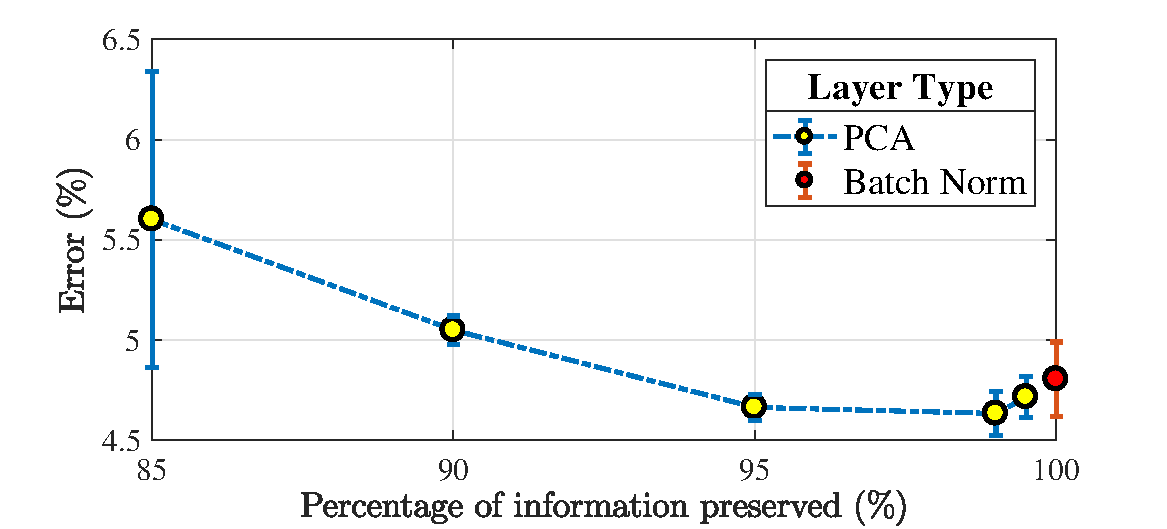
\includegraphics[width=\linewidth]{information.pdf}
}
{%
  \caption{Preserved information VS Performance.}%
}
\capbtabbox[.9\Xhsize]{%
\begin{tabular}{cc}
\hline
Percentage (\%) & Error (\%) \\ \hline
85              & $5.60\pm0.74$  \\ \hline
90              & $5.05\pm0.07$  \\ \hline
95              & $4.67\pm0.06$  \\ \hline
99              & $\mathbf{4.63\pm0.11}$  \\ \hline
99.5            & $4.72\pm0.10$  \\ \hline
100             & $4.81\pm0.19$  \\ \hline
\\
\end{tabular}
}{%
  \caption{Performance Comparison}%
}
\end{floatrow}
\end{figure}

\subsection{Number of EigenVectors VS Performance}

\begin{figure}[!htb]
\begin{floatrow}
\ffigbox[1.1\FBwidth]{%
  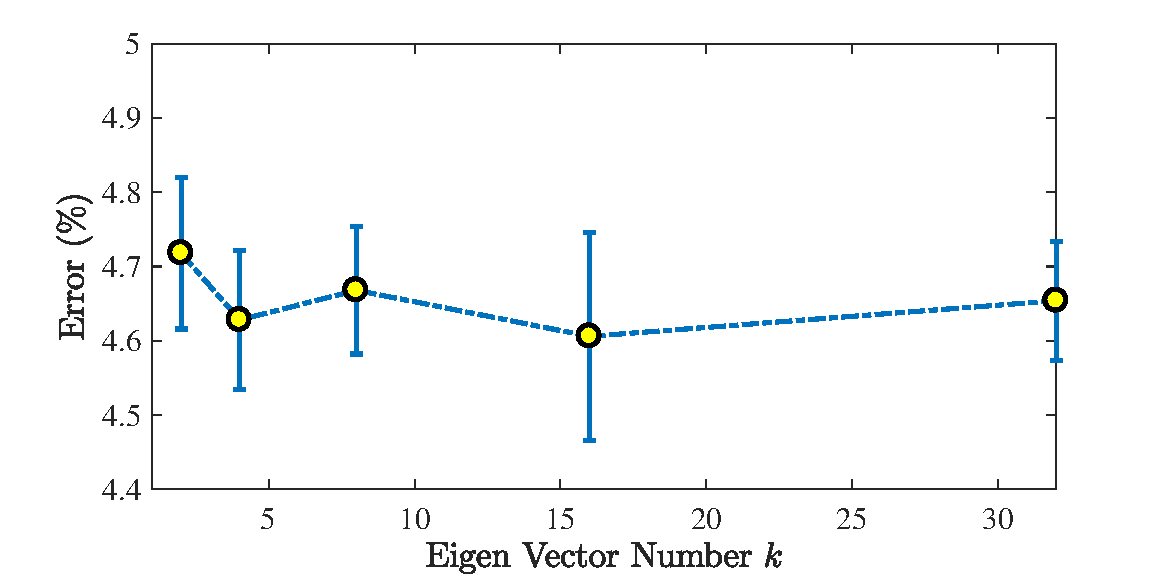
\includegraphics[width=\linewidth]{eig.pdf}
}
{%
  \caption{Eigen-vector No. VS Performance.}%
}
\capbtabbox[.9\Xhsize]{%
\begin{tabular}{cc}
\hline
Eig-vector No. & Error (\%) \\ \hline
2              & $4.72 \pm 0.10$  \\ \hline
4              & $4.63 \pm 0.09$  \\ \hline
8              & $4.67 \pm 0.09$ \\ \hline
16            & $4.61 \pm 0.14$  \\ \hline
32             & $4.65 \pm 0.08$  \\ \hline
\\
\end{tabular}
}{%
  \caption{Performance Comparison}%
}
\end{floatrow}
\end{figure}

\subsection{Number of Power Iterations VS Performance}

\begin{figure}[!htb]
\begin{floatrow}
\ffigbox[1.1\FBwidth]{%
  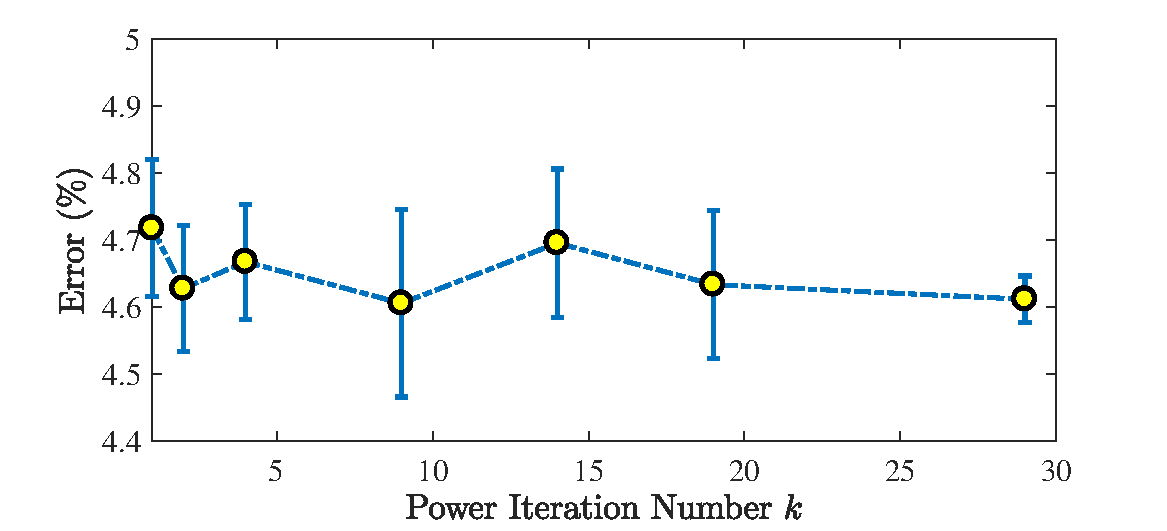
\includegraphics[width=\linewidth]{pi.pdf}
}
{%
  \caption{Power Iteration No. VS Performance.}%
}
\capbtabbox[.9\Xhsize]{%
\begin{tabular}{cc}
\hline
Power Iteration No. & Error (\%) \\ \hline
1              & $4.72 \pm 0.10$  \\ \hline
2              & $4.63 \pm 0.09$  \\ \hline
4              & $4.67 \pm 0.09$  \\ \hline
9              & $4.61 \pm 0.14$ \\ \hline
14            & $4.69 \pm 0.11$  \\ \hline
19             & $4.63 \pm 0.11$  \\ \hline
29             & $\mathbf{4.61 \pm 0.03}$  \\ \hline
\end{tabular}
}{%
  \caption{Performance Comparison}%
}
\end{floatrow}
\end{figure}

\section{Experiment}

In the experiment, within the PCA denoising layer, we remove the noise in the feature maps by only selecting its top-$k$ eigenvectors to reconstruct the input feature maps.
We first reshape the input feature maps $X_{n {\times} c {\times} h {\times} w}$ to $X_{c {\times} nhw}$, and compute the covariance matrix $Var(X) =\frac{XX^{\top}}{nhw-1}$.
The constraint for $k$ is that $\frac{\sum_{i=1}^k\lambda_i}{\sum_{i=1}^n\lambda_i} \geq 0.95$, which means that $95\%$ of the information is preserved and the rest of the information which is lower than $5\%$ is removed. 
In practice, $k$ is relatively small compared with channel number $c$. For instance, on Cifar10 dataset, after the first convolutional layer in ResNet18 which has the channel 64, we observe that \\
more than $95\%$ of the information could be preserved when $k=7$; \\
more than $99\%$ of the information could be preserved when $k=15$; \\
more than $99.5\%$ of the information could be preserved when $k=31$. 

%\begin{table}[!htb]
%\begin{centering}
%\begin{tabular}{|l|c|c|c|c|}
%\hline
%Norm Methods          & BN        & PCA(PI)  & PCA(SVD) & PCA(SVD+PI) \\ \hline
%Minimum Error         & 4.66       & 5.05   & NaN   &\textbf{4.58}\\ \hline
%Mean Error (4) & $4.81{\pm}0.19$ &$5.35{\pm}0.25$ & NaN &$\mathbf{4.67{\pm}0.06}$ \\ \hline
%\end{tabular}
%\caption{CIFAR-10 test errors using ResNet18 (single PCA/ZCA normalization layer).}
%\end{centering}
%\end{table}

\begin{figure}[!htb]
\begin{floatrow}
\ffigbox[0.9\FBwidth]{%
  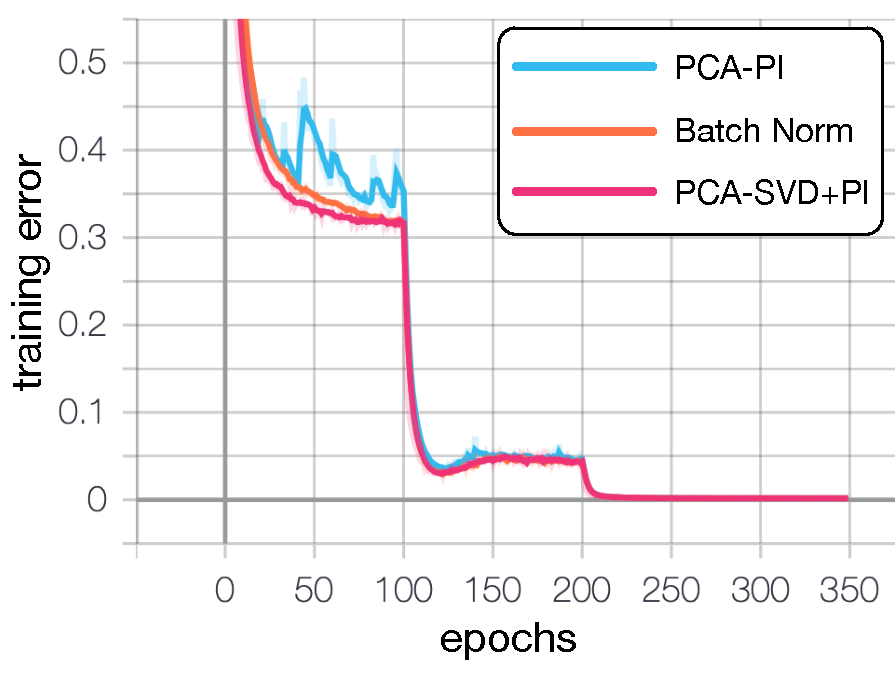
\includegraphics[width=\linewidth]{convergence.pdf}
}
{%
  \caption{Methods VS Performance.}%
}
\capbtabbox[\Xhsize]{%
\begin{tabular}{lcc}
\hline
Methods     & Min Error & Mean Error (5) \\ \hline
BN          & 4.66      & $4.81{\pm}0.19$   \\ \hline
PCA(PI)     & 5.05      & $5.35{\pm}0.25$ \\ \hline
PCA(SVD)    & NaN       & NaN                   \\ \hline
PCA(SVD+PI) & 4.58      & $\mathbf{4.67{\pm}0.06}$ \\ \hline
\\
\\
\\
\end{tabular}
}{%
  \caption{Methods VS Performance.}%
}
\end{floatrow}
\end{figure}


\begin{table}[!htb]
\begin{centering}
\begin{tabular}{|l|c|c|c|c|c|}
\hline
Norm Methods          & BN        & PCA(1 layer)   & ZCA(1 layer)  & PCA(1 block)   & ZCA(1 block) \\ \hline
Minimum Error         & 4.66      &  4.58  &   4.91 &  5.14 &  5.38\\ \hline
Mean Error (4) & $4.81{\pm}0.19$  &  $4.67{\pm}0.06$  & $5.02{\pm}0.28$ & $5.30{\pm}0.12$ & $5.50{\pm}0.10$ \\ \hline
\end{tabular}
\caption{CIFAR-10 test errors using ResNet18 (single PCA/ZCA normalization layer).}
\end{centering}
\end{table}


\medskip
\small
\bibliographystyle{unsrt}
\bibliography{neurips_2019.bib}

\end{document}
